\documentclass[conference]{IEEEtran}
\IEEEoverridecommandlockouts
% The preceding line is only needed to identify funding in the first footnote. If that is unneeded, please comment it out.
\usepackage{cite}
\usepackage{amsmath,amssymb,amsfonts}
\usepackage{algorithmic}
\usepackage{textcomp}
\usepackage{xcolor}
\usepackage{tikz}
\definecolor{titlepagecolor}{cmyk}{.5,.0,.40,.60}

\DeclareFixedFont{\titlefont}{T1}{ppl}{b}{it}{0.5in}

\makeatletter                       
\def\printauthor{%                  
	{\large \@author}}              
\makeatother


\def\BibTeX{{\rm B\kern-.05em{\sc i\kern-.025em b}\kern-.08em
		T\kern-.1667em\lower.7ex\hbox{E}\kern-.125emX}}
	
\begin{document}


\begin{figure}[h!]
	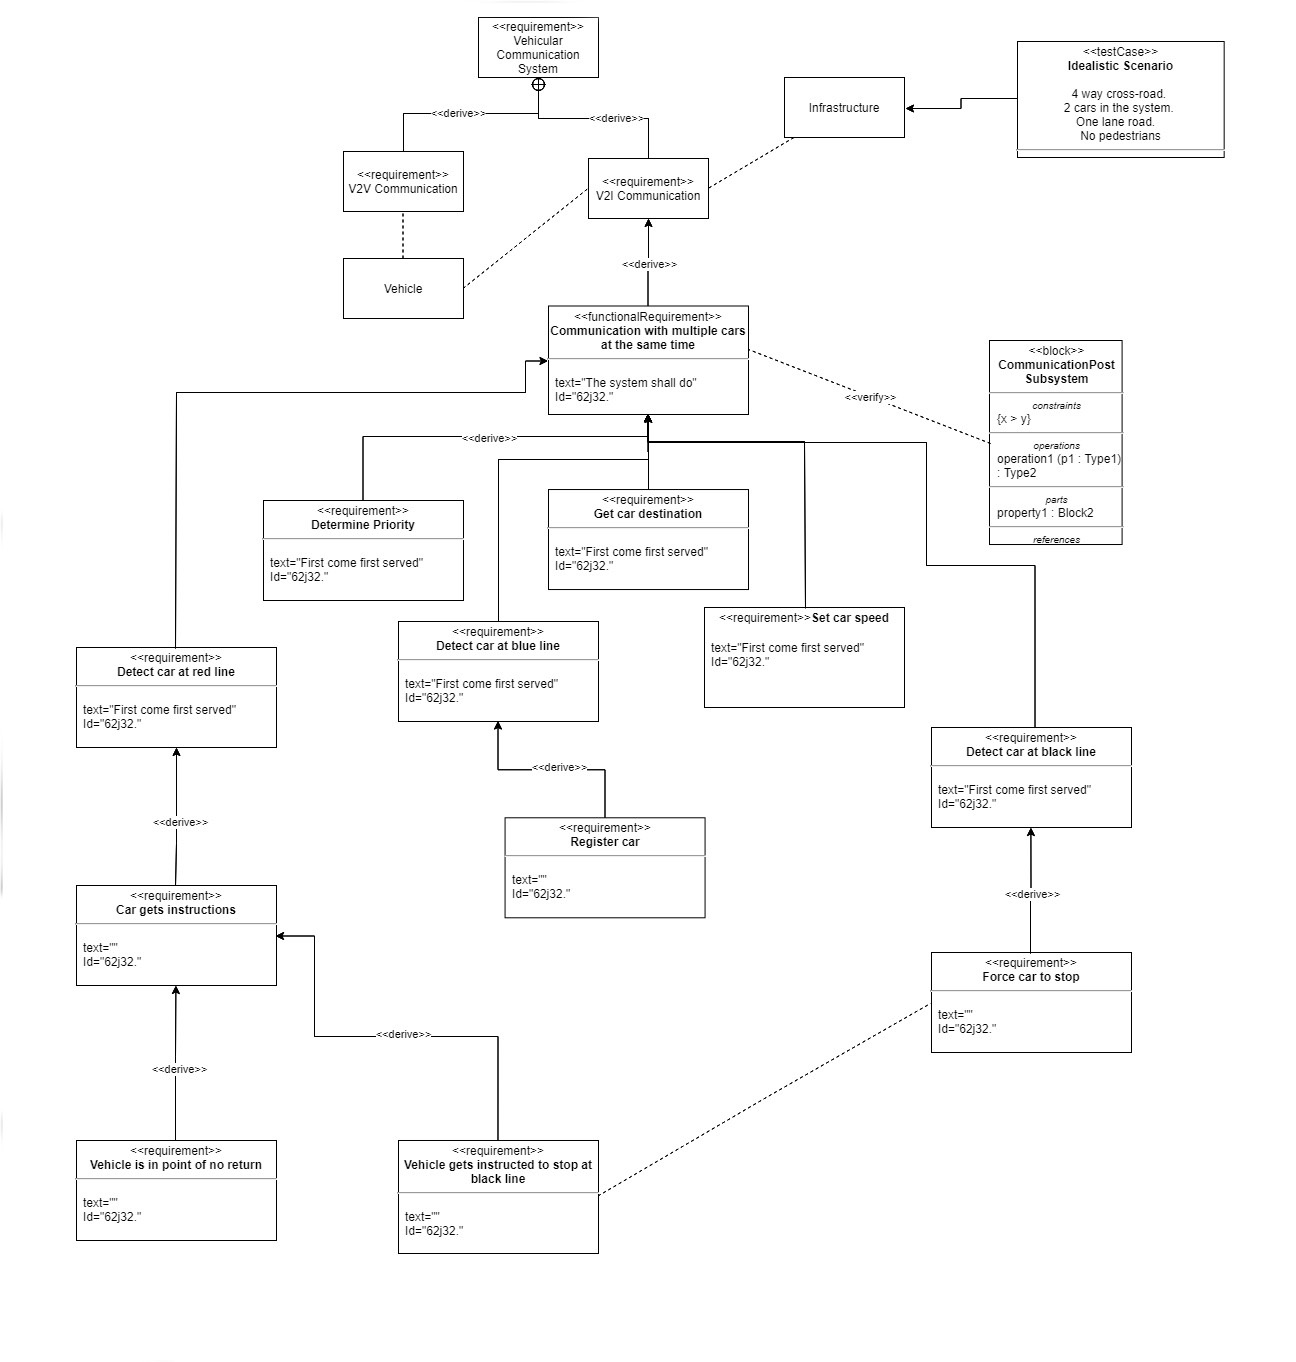
\includegraphics[width=16cm, height=15cm]{Requirement_Diagram}
	\caption{TTEthernet Showcase [5]}
	\centering
\end{figure}
\section{Requirements}
Before any other precedents are set, it is crucial to define and delineate the specific requirements that the project must meet, which will be divided in three parts:
\begin{itemize}
	\item Environmental Requirements
	\item Technical Requirements
	\item Vehicular Requirements
\end{itemize} 

\subsection {Environmental Requirements}
The environment is set to be ideal, which will eliminate a lot of inevitable errors, but an effort will still be made into making this project compatible with the real world, at least conceptually. The environment would essentially be composed of a single crossroad in which the scenarios would take place. The elements of the crossroad are as follows: There are four separate bidirectional roads (each with a single detectable lane) which all meet in the middle. Each road will \\  \\  \\  \\  \\  \\  \\  \\  \\  \\  \\  \\ \\  \\  \\  \\  \\  \\  \\  \\  \\  \\  \\  \\  \\  \\  \\  \\  \\  \\  \\  \\  \\  \\  \\  be tagged as  either North, West, South or East and it would be done so liberally, meaning that the position of the roads do not have to point toward, for example, true North. That would mean that every other following crossroad would also be marked as such, although our scenarios will only be contained in a single one. Cutting through the roads will be vertical lines that would be used as indicators, or just simply markers, that would mark the distance from the line - to the center. There are three such lines, each with their own color code (blue, red and black) and the full details of their nature are described below. 
\subsection{Technical Requirements}
The main technology behind the project will be a "communication box", although its usage will be described further below. The following metrics have to be met:
\begin{itemize}
	\item each road is at least 200m long
	\item there is 150m distance between the blue line and the black line
	\item however, there is 75m between the blue line and the red line
	\item there must be a buffer distance of ~5 meters from the red line
	\item the scheduling time constraint is limited to 5 seconds
	\item each car would have their speed limited to 50 km/h, fixed, after passing the blue line
\end{itemize} 
\subsection{Vehicular Requirements}
The vehicles are expected to run in quite a decentralized fashion. Since the environment is set to be ideal, we presuppose that there will be universal standards put in place. The vehicles would use the communication box as a secondary source of information, while the road as a primary one, and the standards are there to define how exactly the vehicles would interpret certain data points. But what makes the vehicles particularly "decentralized" is the fact that the decision making process is left to them, i.e. the communication box cannot interfere with the decision making process.
\begin{figure}[h!]
	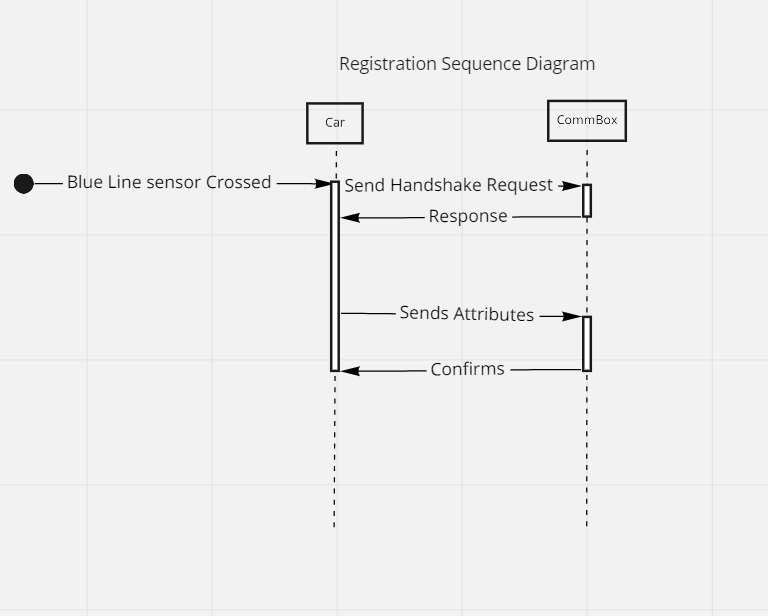
\includegraphics[width=8cm, height=6cm]{Sequence_diagram_init_comm}
	\caption{Sequence Diagram}
	\centering
\end{figure}


\section{Initial Communication}
The initial communication between the vehicles and the communication box is established the moment the vehicle detects the initial vertical line (blue line). The vehicle then detects the communication box trough a Fire and Forget UDP signal, after which it sends a handshake request and awaits a response. Once the vehicle receives a response and establishes a successful first connection, it proceeds to send information about its attributes:

\begin{itemize}
	\item current speed
	\item destination (nothing too data heavy, it would be as simple as choosing the Northern or Southern road, for example)
	\item size of the vehicle (for safety, collision-detection purposes)
\end{itemize} 
Once the attributes have been received by the communication box, the vehicle proceeds by executing on further information sent by the connection requests that follow after, specifically: how the speed of the vehicle needs to be configured (either lowered or sped-up), in which direction the vehicles is allowed to drive and any information necessary to avoid collision with other vehicles. These instructions are memorized and put in/taken from the heap of the communication boxes on-board memory and scheduler. The scheduler allows for the simultenious communication with more than one vehicle at one time.
\begin{figure}[h!]
	\includegraphics[width=6cm, height=6cm]{data_collection}
	\caption{Data Collection Diagram}
	\centering
\end{figure}
\section{Scheduler}
 The scheduler is best described with these diagrams: 
 \begin{figure}[h!]
 	\includegraphics[width=8cm, height=7cm]{Mutex}
 	\caption{Mutex Diagram}
 	\centering
 \end{figure}
 \begin{figure}[h!]
	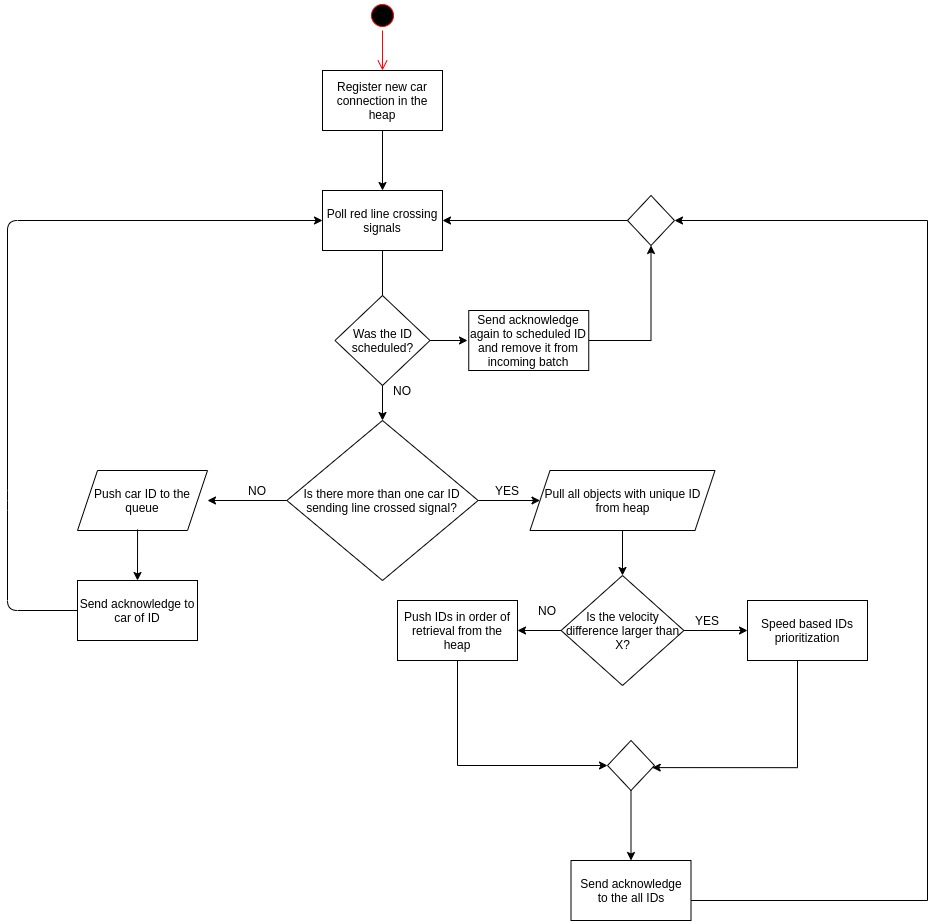
\includegraphics[width=8cm, height=8cm]{Activity_diagram_for_scheduler}
	\caption{Activity Diagram for the Scheduler}
	\centering
\end{figure}
\end{document}
